%  ========================================================================
%  Copyright (c) 1985 The University of Washington
%
%  Licensed under the Apache License, Version 2.0 (the "License");
%  you may not use this file except in compliance with the License.
%  You may obtain a copy of the License at
%
%      http://www.apache.org/licenses/LICENSE-2.0
%
%  Unless required by applicable law or agreed to in writing, software
%  distributed under the License is distributed on an "AS IS" BASIS,
%  WITHOUT WARRANTIES OR CONDITIONS OF ANY KIND, either express or implied.
%  See the License for the specific language governing permissions and
%  limitations under the License.
%  ========================================================================
%

% Documentation for University of Washington thesis LaTeX document class
% by Jim Fox
% fox@washington.edu
%
%    Revised for version 2015/03/03 of uwthesis.cls
%    Revised, 2016/11/22, for cleanup of sample copyright and title pages
%
%    This document is contained in a single file ONLY because
%    I wanted to be able to distribute it easily.  A real thesis ought
%    to be contained on many files (e.g., one for each chapter, at least).
%
%    To help you identify the files and sections in this large file
%    I use the string '==========' to identify new files.
%
%    To help you ignore the unusual things I do with this sample document
%    I try to use the notation
%       
%    % --- sample stuff only -----
%    special stuff for my document, but you don't need it in your thesis
%    % --- end-of-sample-stuff ---


%    Printed in twoside style now that that's allowed
%
 
\documentclass [11pt, proquest] {uwthesis}[2016/11/22]
 
%
% The following line would print the thesis in a postscript font 

% \def\bibpreamble{\protect\addcontentsline{toc}{chapter}{Bibliography}}

\setcounter{tocdepth}{1}  % Print the chapter and sections to the toc


% ==========   Local defs and mods
%

% --- sample stuff only -----
% These format the sample code in this document
\usepackage{hyperref} 
\usepackage{alltt}  % 
\usepackage{fontspec}
\usepackage{xspace}
\usepackage{microtype}
\usepackage{graphicx}
\usepackage{subfigure}
\usepackage{booktabs} % for professional tables
\usepackage{graphicx}
\usepackage{tikz}
\usepackage{amsmath}
\usepackage[english]{babel}
\usepackage{blindtext}
\usepackage{bbm}
\usepackage{textcomp}
\usepackage{ulem}
\usepackage{tabularx}
\usepackage{enumitem}
\usepackage{xcolor}
\usepackage[font=small,skip=-0pt]{caption}
% \setmainfont[Ligatures=TeX]{DENG.TTF}
\newenvironment{demo}
  {\begin{alltt}\leftskip3em
     \def\\{\ttfamily\char`\\}%
     \def\{{\ttfamily\char`\{}%
     \def\}{\ttfamily\char`\}}}
  {\end{alltt}}
 
 \newcommand{\pbox}{Parameter Box\xspace}
 \newcommand{\phub}{Parameter Hub\xspace}
 \newcommand{\plink}{Parameter Link\xspace}
 \newcommand{\pseries}{Parameter\xspace}
 \newcommand{\azure}{\textcolor{azureC}{Azure}\xspace}
\newcommand{\ectwo}{\textcolor{ec2C}{EC2}\xspace}
%\newcommand{\marcopolo}{Marcopolo\xspace}
\newcommand{\marcopolo}{ProbeEmbed\xspace}
\newcommand{\ha}{AggEngine\xspace}
\newcommand{\mlha}{2LHA\xspace}
\newcommand{\strongrandom}{Balanced Random\xspace}
\newcommand{\autoplink}{Autotune\xspace}
\newcommand{\code}[1]{\texttt{\small{#1}}}
\newcommand{\strongbaseline}{strong baseline\xspace}

% metafont font.  If logo not available, use the second form
%
% \font\mffont=logosl10 scaled\magstep1
\let\mffont=\sf
% --- end-of-sample-stuff ---
 



\begin{document}
 
% ==========   Preliminary pages
%
% ( revised 2012 for electronic submission )
%

\prelimpages
 
%
% ----- copyright and title pages
%
\Title{Towards More Efficient Communication for Distributed Learning Systems}
\Author{Liang Luo}
\Year{2020}
\Program{Computer Science and Engineering}

\Chair{Luis Ceze}{Professor}{Computer Science and Engineering}
\Signature{Arvind Krishnamurthy}
\Signature{Zachary Tatlock}
\Signature{Eric Klavins}
\Signature{Jacob Nelson}


\copyrightpage

\titlepage  

 
%
% ----- signature and quoteslip are gone
%

%
% ----- abstract
%


\setcounter{page}{-1}
\abstract{%
The explosion of data volume and ever-increasing speed of accelerators shifts the bottleneck of large-scale distributed learning tasks from computation to communication. We observe significant pressure on the communication backends of various mainstream learning systems in multiple environments. Achieving efficient larger scale learning relies on more effective communication plane.

We provide detailed analyses that root-causes the reasons affecting the efficiency of these systems in the context of different environments. We pinpoint bottlenecks from the software, hardware and network infrastructure stacks.  

We show how these obstacles can be overcome with a systematic codesign of a streamlined communication stack, a balanced hardware and cluster configuration with the distributed training workload, together with awareness of network topology and environment. We show this series of  approaches, named \pbox, \phub and \plink, accelerates distributed training from small clusters to datacenters and all the way to the commercial clouds while allows for variable degree of transparency: the \pseries series enables solutions with no code change required to full customization of hardware.
}
 
%
% ----- contents & etc.
%

%\listoftables  % I have no tables
 
%
% ----- glossary 
%
%\acknowledgments{% \vskip2pc
  % {\narrower\noindent
%  The author wishes to express sincere appreciation to
%  University of Washington, where he has had the opportunity
%  to work with the \TeX\ formatting system,
%  and to the author of \TeX, Donald Knuth, {\it il miglior fabbro}.
  % \par}
%}

%
% ----- dedication
%
\dedication{\begin{center}Thank you to my parents, Changyi and Yanan, for your endless love and support.

Thank you to my academic advisers, Luis Ceze and Arvind Krishnamurthy, for patiently guiding me through the process.

Thank you to this committee for keeping me on track. 



Thank you to my friends for the joy and laughter in the journey.


Special thanks to Novak Djokovic, we may never meet, but you bring the inspirations on and off court.


\end{center}}

\section{Introduction}
Today, learning systems have gained significant attention in the literature for the overwhelming popularity of machine-learning (ML) related workloads. Most of work to date in the systems and architecture community has focused on improving the efficiency of evaluating trained models. This makes sense given that a model is trained only once but can be used many times for inference. However, arriving at a trained model frequently requires experimentation, and thus multiple training runs, each of which may take days. Accelerating the training process lets ML scientists iterate faster and design better model.

Traditionally, training has been viewed as a compute-bound problem, best done in a single large compute node with many accelerators. However, the ever-growing data volume pushes for monster-sized models, a scale even the exponentiation of compute power growth in single device couldn't handle. As ML models get bigger, training time gets prohibitively longer. Timely training requires exploiting parallelism with a distributed system.

\begin{table}
\centering
\begin{tabular}{|c|c|c|c|c|}
  \hline
  Models & Complexity & Size & Time & Configuration \\
  \hline
  Linear Regression~\cite{seber2012linear} & O($D^3+ N^2D$) & Small & Short & CPU \\
  \hline
  SVM~\cite{wang2005support} & O($N^2D^2$) & Small & Short & CPU \\
  \hline
  GBDT~\cite{friedman2001greedy} & O($TLFN$) & Small & Short & A few CPUs \\
  \hline
  \hline 
  AlexNet~\cite{alexnet}   & 0.0058 & 48M & 6 days  & 2x GTX 580\\
  \hline
  ZFNet~\cite{ZFNet}   & 0.0062  &  $\approx$48M  & 12 days  & GTX 580\\
  \hline
  VGGNet~\cite{VGGNet}   & 0.12  & 137M & 15 days & 4x Titan Black\\
  \hline
  GoogleNet~\cite{GoogleNet}   & 0.03  & 9M & 7 days & A few GPUs\\
  \hline
  ResNet~\cite{RESNET}   & 0.117 &  58M & 21 days & 8x GPUs\\
  \hline
  Xception~\cite{Chollet_2017}  & 5.0  & 22M & 30 days & 60x K80\\
  \hline
  \hline
  BERT~\cite{bert}  & 3.8 & 340M & 4 days & 16x TPUs v2 \\
  \hline
  GPT-2~\cite{GPT2}  & 248 & 1.5B & 7+ days~\cite{gpt2Time} & 256x TPUs v3 \\
  \hline
  \hline
%  Device Placement~\cite{mirhoseini2017device} 2017 & - & 27 hours & 80 GPU nodes  \\
%  \hline
  NAS~\cite{zoph2016neural}  & 31 & 86M & 28 days & 800 K40 GPUs\\
  \hline
  AlphaGoZero~\cite{silver2016mastering}  & 1800 & - & 1 day & 5000x TPUs \\
  \hline
\end{tabular}
\caption{A few representative machine learning techniques and models that support increasingly complex tasks (trees, support vector machines, neural networks) and their complexities to train (pfs-day, or days to train computing at 1 PFlop/s. 1PF/s roughly corresponds to 64 Tesla V100 GPUs FP32, or 8 with mixed-precision FP16, running at peak throughput), and their reported training time and the machines they are trained on. We used the same method of estimating complexity as in the original OpenAI blog post~\cite{AIandCom3:online} for the additional models in the table. $D$: features. $N$: samples. $L$: leaves per tree. $T$: number of trees to build.}
\label{table:trend}
\end{table}

Table~\ref{table:trend} gives a taste of the evolution of machines learning models/techniques: they are getting increasingly more demanding in terms of compute resources, such that the use of hundreds or even thousands of machines and accelerators for weeks is commonplace. 




The most common way of exploiting parallelism, ``data'' parallelism, consists of a computation-heavy local computation phase and a communication-heavy parameter exchange phase. Efficient distributed training involves optimizing both stages. Many past work demonstrate the solution of accelerating these processes by building specialized hardware clusters with fast interconnects ~\cite{DBLP:journals/corr/abs-1711-00489, You:2018:ITM:3225058.3225069, DBLP:journals/corr/abs-1711-04325,jia2018highly,DBLP:journals/corr/abs-1811-05233,sun2019optimizing, ImageNetIn1Hour, firecaffe, phubsocc}. While the results are encouraging, as we shall see, faster hardware is not panacea: the unstreamlined software stack and unbalanced compute to communication resource allocation prohibits utilizing full capability of the hardware, and the compute units are more likely than not waiting on the network because the latter simply cannot keep up (Figure~\ref{fig:clusterOverhead}). We expect the problem not going away on its own, because of the observed trend at which the network capability is growing is significantly outpaced by that of the compute resources (Figure~\ref{fig:accthroughput}).  


\begin{figure}
	\centering
	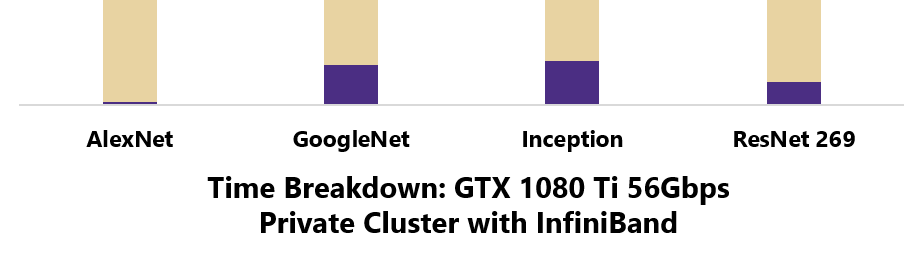
\includegraphics[width=.5\linewidth, trim=6 1 3 3,clip]{Figures/clusteroverhead.png}
	\caption{Even with a fast, small-scale cluster, communication still takes most of the time duration training, wasting compute resources.}
	\label{fig:clusterOverhead}
\end{figure}

\begin{figure}
	\centering
	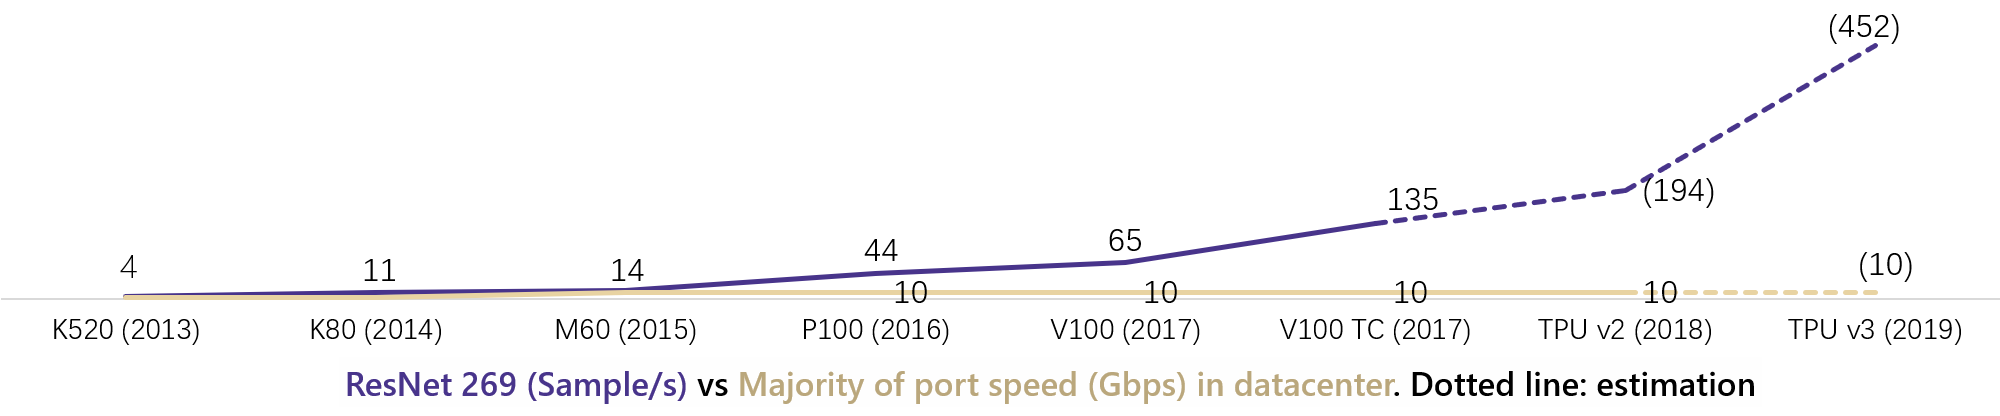
\includegraphics[width=\linewidth, trim=2 3 3 3,clip]{Figures/computevscomm.png}
	\caption{Throughput for an industry standard benchmark (ResNet) has seen an improvement of 35x, and is estimated to increase by 100x with latest accelerators. GPU performance tested with MxNet on EC2. TPU throughput estimated based on TensorCore's measured performance. Estimation for majority of the port speed of datacenters is based on Cisco study~\cite{CISCOMarket}. Only until very recently did the public cloud start offering 100Gbps bandwidth instances on standalone VMs~\cite{Introduc9:online, NewC5nIn6:online}}.
	\label{fig:accthroughput}
\end{figure}

To tackle these problems, a comprehensive codesign of software stack and hardware configuration is required. To that end, we provide a template for speccing an entity called \pbox that provides the near perfect communication to computation balance for acting as a parameter server in a distributed training job, and a companion piece of software, \phub that streamlines handling over gradient  transfer, aggregation and model optimization by carefully extracting locality inside a physical host and latency hiding. 

While \pbox and \phub are effective, it is important to understand accelerating training in these specialized, privately-owned clusters does not complete the story: first, those hardware setups require steep investment and only a few have that luxury; second, since it is much easier to thoroughly optimize the entire stack in private clusters as we have control over the entire system, some optimizations are not always possible to be applied universally.

An alternative to owning a private cluster is renting VMs from the public cloud, which has become a popular, more accessible approach. Currently, all major cloud providers offer racks of nodes with specialized accelerators (such as GPUs, TPUs, and custom FPGAs)~\cite{GoogleCl74:online,MachineL50:online,DeepLear23:online,sagemaker,brainwave,Jouppi:2017:IPA:3079856.3080246,222611} for ML workloads. But at the same time, scalable training in the public cloud isn't just a straightforward application of \pbox and \phub optimizations.

\begin{figure*}[t!]
	\centering
	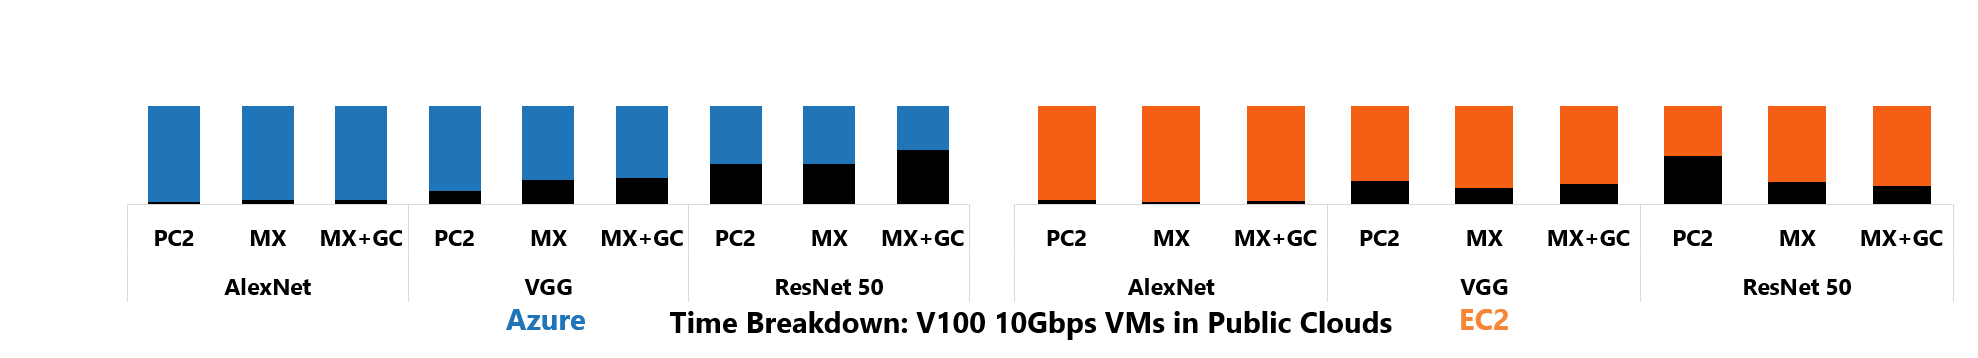
\includegraphics[width=.9\linewidth, trim=6 1 3 3,clip]{Figures/cloudoverhead.png}
	\caption{Even with state of the art training frameworks and recent optimizations, up to 90\% of time during cloud-based training of popular models is wasted explicitly waiting on the network in the public clouds.}
	\label{fig:cloudOverhead}
\end{figure*}


Even with modern frameworks and recent optimizations 
(e.g., gradient compression and quantization~\cite{lin2017deep, cntk1bt, lim20183lc}, latency-hiding~\cite{poseidon, jayarajan2019priority,hashemi2018tictac}, optimized communication libraries~\cite{facebook35:online, Operatio73:online, dmlcpsli50:online} and large batch optimizations~\cite{ImageNetIn1Hour}), distributed training at scale on the public cloud still incurs high overhead: up to 90\% of total training time can be wasted waiting on the network (Figure~\ref{fig:cloudOverhead}). Further, existing solutions so far focus solely on addressing the \textit{bandwidth} bottleneck, and ignores cloud-specific challenges: the hierarchical network structure in datacenter breaks the usual assumption of link speed being uniform; multi-tenancy and the dynamic nature of the cloud traffic cause high variation in performance. All these add to the complexity of scaling up distributed training and can render existing solutions less effective. 

Accelerating cloud-based distributed training thus requires paying attention to a third dimension (apart from software and hardware): the environment. First, we need an aggregation mechanism that is appropriate for network topologies that display bandwidth oversubscription, and that makes appropriate use of underprovisioned links.  Second, we need to be able to identify the underlying network topologies and bandwidth/latency constraints (or collectively, locality) even if the public cloud does not expose such information.  Finally, we need communication schemes that can react to changing network conditions, especially in the presence of interfering traffic generated by other tenants. Our solution is collectively called \plink, an optimized, locality-aware system that uses a fitted hierarchical aggregation scheme to extract locality from the underlying datacenter network, based on end-to-end network probes and dynamic network load.

With \pbox, \phub and \plink, we complete the picture of accelerating machine learning of all kinds, ubiquitously. In the following sections, we start with an overview of the mechanism of distributed training, then we walk through each of the proposed solution in detail. We show how specific optimizations adopted target directly at the bottlenecks in each scenario and lead to end-to-end speedup in real-world learning tasks.
\section{Background}
We now establish conventions used in this paper, and familiarize the reader with basic concepts for distributed training.


\subsection{Training a ML model}
Different types of models may appear to have different ways of training, but sitting at the center of most models is the common notion of parameters and gradients. Parameters are the goals: they define the ultimate models; gradients are the means: they are derived with respect to parameters, and guide how parameters should be adjusted to minimize the errors together with a learning rate, usually in an iterative manner, using the technique (or its variant) gradient descent~\cite{subgradient,DBLP:journals/corr/Ruder16}. 

To illustrate the training process, we use the example of training a deep learning (DL) model, or a deep neural network (DNN), for its popularity. We will continue to explain in the context of DL models throughout this paper for consistency. Modern DL models can have hundreds of \textit{layers} making up multi-megabyte-size \textit{models}. The training process has three phases. In the \textit{forward pass}, a prediction is generated for an input. In the \textit{backward pass}, the prediction is compared with a label to calculate prediction error; then, through \textit{backpropagation}~\cite{backprop}, the gradient for each parameter
is calculated with respect to this error. The model is then \textit{updated} using these gradients, often using a variant of the gradient descent optimization algorithm. Each Computation is often done on GPUs or other accelerators suited to regular data-parallel operations, processing a batch of samples at once (\textit{minibatching}).
%Multiple examples are processed in each GPU simultaneously in a single \emph{minibatch} which typically contains tens to hundreds of samples. 
%Each GPU processes multiple examples simultaneously in a \emph{minibatch} which typically contains tens to hundreds of samples. 

\begin{figure}[t!]
	\centering
	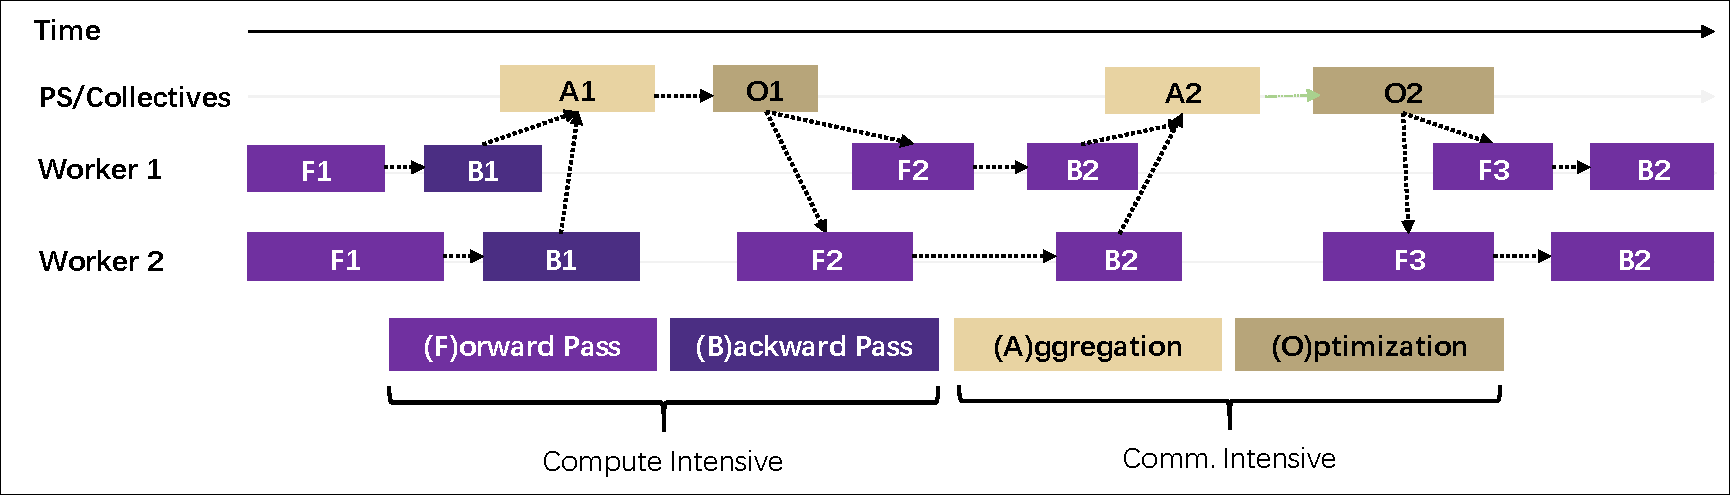
\includegraphics[width=\linewidth, trim=2 3 3 3,clip]{Figures/distributedtraining.pdf}
	\caption{A few iterations of distributed training pipeline of neural networks.}
	\label{fig:distributedtraining}
\end{figure}

\subsection{Distributed Training}
Broadly speaking, there are two extremes in terms of paradigms in distributed training: \textit{data} parallelism and \textit{model} parallelism, and many hybrid systems strike a balance between this two.

In data parallelism, there is the notion of \textit{workers} and \textit{servers}, two non-exclusive roles a node can take. Training data is prepartitioned to each individual workers, and servers store the current model parameters in a sharded manner. In the computation phase of each iteration, no data is exchanged until all workers derive the gradients; gradients are then sent to servers for processing.

In model parallelism, instead of partitioning training data, the model itself is being partitioned. This is handy because the multi-layer of modern DL models and well-defined dependencies make it simple to partition the model to different nodes. A piece of data then follows through the entire system, as if in the single node training case, except that it crosses node boundaries.

This paper mainly focuses on data parallelism, as it is the default choice in many frameworks and practices. The distributed training process (Figure~\ref{fig:distributedtraining}) using data parallelism is different in a few ways from training within a single node.
%First, a mean gradient is calculated for each minibatch in each GPU. %
First, a mean gradient is calculated across all minibatches in each machine. Then, the mean of the gradients from each machine is calculated. Finally, the model is updated based on that mean, new parameters are broadcast to each machine and GPU, and the next batch is trained. This paper focuses on optimizing calculation of both the mean gradient across machines and the subsequent model update (or \textit{parameter exchange}). Note that gradient aggregation and model optimization are both element-wise operations.

%n the second, each worker also stores a shard or replica of the global model; model updates are done through collective communication operations involving all machines.

The process described here is \textit{synchronous training}, where all machines and GPUs execute a new minibatch simultaneously and update the model based on the gradients in the current iteration. It is also possible to train asynchronously~\cite{tensorflow,revisitSGD,GeePS,recht2011hogwild,projectAdam,googleDNN}, sacrificing reproducibility for a potential throughput increase. %updating the model with the gradient from each GPU's minibatch with little or no synchronization among machines; this can improve throughput in some situations but may limit repeatability and debuggability. 
We focus on synchronous training due to its simplicity and commonality in industry, but our techniques can also benefit asynchronous training.

\begin{figure}[t!]
	\centering
	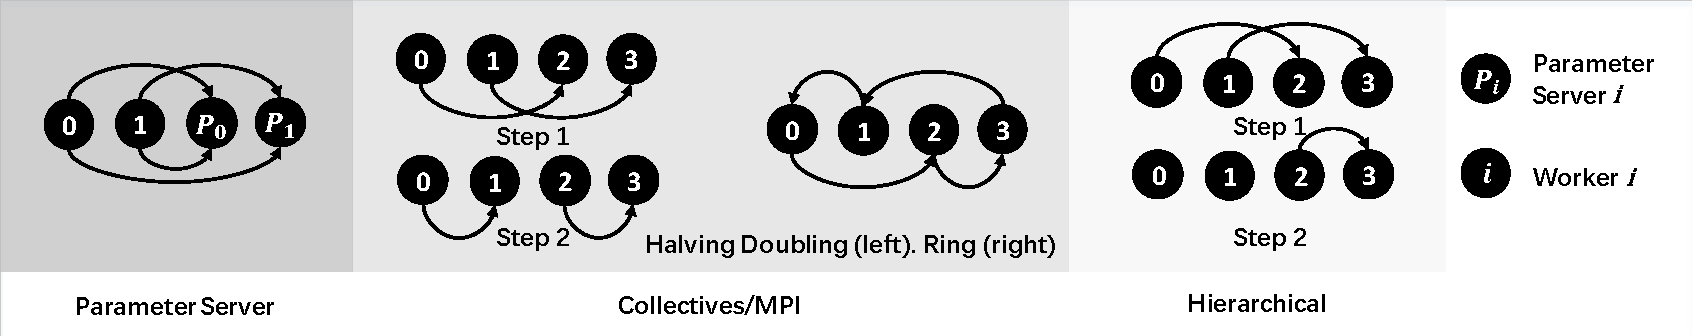
\includegraphics[width=\linewidth, trim=2 3 3 3,clip]{Figures/aggregationapproaches.pdf}
	\caption{Aggregation is commonly done with one of the three prevailing paradigms, parameter server, collectives all-reduce, and hierarchical aggregation in practice.}
	\label{fig:aggregationapproaches}
\end{figure}

\subsection{Distributed Training is Here to Stay}
Faster and more powerful accelerators (most notably TPUs~\cite{Jouppi:2017:IPA:3079856.3080246} and Nvidia DGX~\cite{AIResear61:online}) open up the possibility of training in a single device. It all of sudden seems plausible to build a ``supercomputer'' for training, which completely eliminates the need for costly communication. 

Unfortunately, building a training supercomputer does not avoid the problem of insufficient compute resources, but only delay it, for at least two reasons. From a historic perspective, it never happens that there is a surplus in the compute power when it comes to new models, as shown in Table~\ref{table:trend}: scientists can always find models whose complexities are well beyond reach of a single device, which frequently ended up being trained in a distributed fashion: the use of a single device (e.g. DGX) is not because that single device covers all the need, but rather the lack of additional devices. From an architecture perspective, compute density cannot scale forever as many hard limits are imposed on the number of transistors to fit on a fixed area, including physical effects and cooling constraints. When near these limits, it gets prohibitively difficult to build faster chips within a confined area. 

On the other hand, any training that spans device boundary, not necessarily machine boundary, can be classified as distributed training, and the communication medium need not be limited to conventional network media, but can also include device buses. With this broad view, distributed training is inherent in deep learning. In fact, many have already started looking into optimization of inter-device communication within a single machine~\cite{wang2019blink}. %at each hierarchy (GPU vs PCI-E, Node vs Ethernet), we can observe large gap between the bandwidth of communication and compute. 

\subsection{Gradient Aggregation: Common Practices}
In a loose taxonomy, collecting gradients for aggregation is commonly done with one of the following paradigms (Figure~\ref{fig:aggregationapproaches}).


\begin{figure}[t!]
	\centering
	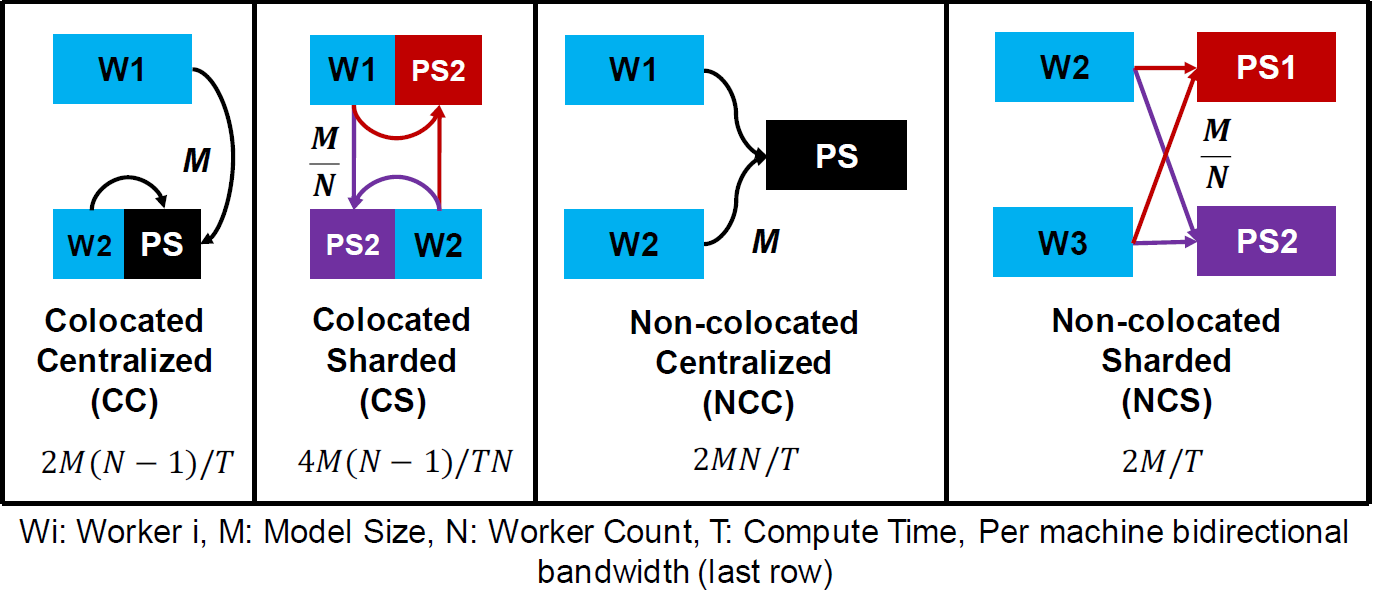
\includegraphics[width=.7\linewidth, trim=2 3 3 3,clip]{Figures/pssetups.PNG}
	\caption{Aggregation is commonly done with one of the three prevailing paradigms, parameter server, collectives all-reduce, and hierarchical aggregation in practice.}
	\label{fig:pssetups}
\end{figure}

\noindent\textbf{Parameter Servers (PS)}~\cite{ps0,ps1,ps2,ps3, phubsocc, phubsysml, poseidon,cui2016geeps}. %Nodes are assigned the role of \textit{workers} or \textit{servers}. 
PSs are key-value stores, where keys and values represent the model's layer IDs and weights. PSs can be centralized or sharded. In each iteration, all workers update the model stored in PSs with their locally-produced gradients. PS configurations primarily differ along two axes: colocated (C) versus non-colocated (NC), and centralized (C) versus sharded (S). %In a colocated setting, a PS process can run with worker processes in the same machine. In a non-colocated setting, a machine is dedicated to a worker or a PS process.  
A PS setup is colocated if a worker and a server process share the same physical machine. A PS setup is centralized if a single PS process handles all keys; and a sharded setup load-balances keys across multiple PS processes.
%A centralized PS stores the entire model, whereas each sharded PS stores only a partition of the keys in the entire key space. The size of each partition is usually balanced by the available hardware resources. 
During synchronization, each worker sends and receives model updates from each PS process. Figure \ref{fig:pssetups} illustrates the four combinations of choices from these two axes: Colocated Centralized (CC), Colocated Sharded (CS), Non-colocated Centralized (NC) and Non-colocated Sharded (NCS).

In general, sharded PSs scale better at higher hardware costs. Colocated PSs reduce total data movement on the network by $\frac{1}{N}$ with $N$ workers participating: the update for the partition of the model assigned to a colocated PS need not go through the network. While many frameworks default to CS configurations~\cite{MXNetont0:online, Distribu25:online}, in a colocated setup the PS process interferes with the training process, because both are contending for network and processing resources. Specifically, compared to NC PSs, \textit{each network interface must process roughly 2x the network traffic, because both the colocated worker and PS processes must send and receive model updates from remote hosts}, creating a major bottleneck in network-bound distributed training. 

\noindent\textbf{Collective AllReduce (CA)}~\cite{Sack:2011:SCM:2522220,Thakur:2005:OCC:2747766.2747771,collectivesOptimization,blum2000architectures,bala1995ccl}. Popular in the context of MPI, all nodes in CA participate in the communication, usually running symmetric tasks. The end goal of CA is that all nodes have a globally-reduced copy of the data. Widely used CA in training deep learning models include halving-doubling~\cite{ImageNetIn1Hour}, ring and double binary tree~\cite{Operatio73:online, Sergeev2018HorovodFA}.

Gradient aggregation can be \textit{flat} (e.g., use of PSes and CAs are generally flat) or \textit{hierarchical} (Hierarchical Aggregation, HA), which refers to the generic technique of aggregating data in multiple steps, from local to global. Exemplar usage of HA in the distributed training context include~\cite{firecaffe,choblueconnect,Geng:2018:HHP:3229543.3229544,sysmlblueconnect}, though in the context of proprietary networks. HA is highly flexible and supports mix and matching of multiple aggregation paradigms~\cite{topoawarempi, cool}.

This paper focuses on the discussion of building efficient PSs, but most of the techniques still apply to accelerating CAs as well. 

\subsection{More Efficient Distributed Training: Prior Arts}
Approaches to accelerating distributed training can be classified into one of the broad categories in the current literature.

\noindent\textbf{Synchronize less often}. One way to achieve a lower synchronization frequency is to oversubscribe GPUs. This can be done by using a very large batch size, fully utilizing GPU memories, making GPU compute the bottleneck~\cite{Nowanyon13:online, ImageNetIn1Hour, sridharan2018scaleout, jia2018highly}. Large batch sizes reduce communication frequency. However, this eliminates the potential of achieving a larger speedup with a fast communication plane. For example, with ResNet-50, ~\cite{Shen2018NexusA} shows only 10 samples are needed to fully utilize a recent GPU. This means the computation of large batches can be further spread to more GPUs, provided that communication overhead is low. Further, large batch optimization is also not universally available (requiring GPUs with large memory) and may be subject to worse generalization~\cite{keskar2016large}.

Orthogonal to large batch optimization, another line of work target at less synchronization tunes the consistency model of distributed training, with relaxed consistency~\cite{DBLP:journals/corr/DaiKWHGX14,SSP,BSP,Wei:2015:MCC:2806777.2806778,Litz,xie2018orpheus,wang2018adaptive}. Generally, these relaxed consistency models do not mandate a strict barrier for synchronization at iteration granularity, and instead, allows for staleness in the model and a potential different view of model from each worker, removing the synchronization overhead from the critical path. However, these methods suffer from difficulty in reproducing the models. 

\noindent\textbf{Send less data}. Sending less data accelerates distributed training in a bandwidth-bound environment, and can be achieved through (1) lossless compression~\cite{burtscher2009fpc}; (2) lossy compression, removing redundancy in the SGD algorithm~\cite{lin2017deep}; (3) quantizing update gradients to low bit representations and locally apply residual errors~\cite{cntk1bt, lim20183lc} and (4) decomposing large update matrices~\cite{projectAdam,poseidon,xie2015distributed} and reconstructing at destination. These methods either trade more computation for less communication, or risk affecting the final convergence accuracy of the model, and both of which may turn out \textit{increasing} the total wall clock time required to reach the target accuracy.

\noindent\textbf{Build faster clusters}. Another series of work involves building specialized hardware clusters for distributed training with quick interconnects to tackle communication bottlenecks~\cite{DBLP:journals/corr/abs-1711-00489, You:2018:ITM:3225058.3225069, DBLP:journals/corr/abs-1711-04325,jia2018highly,DBLP:journals/corr/abs-1811-05233,sun2019optimizing, ImageNetIn1Hour, firecaffe}. While the results have been encouraging, these approaches demand steep investments and are not available to everyone.

\noindent\textbf{Hide communication latency}. Most modern frameworks encode the model being trained as a dataflow graph. An operator is executed as soon as its dependencies are resolved, and this allows overlapping of communication and computation during the backpropagation stage of distributed training. Some work even attempt to reprioritize sending of first layers over later layers to deal with this priority inversion problem. Notable applications of this idea include~\cite{hashemi2018tictac, prioritybased, poseidon, 10.1145/3341301.3359642}. However, communication latency hiding has severe limits: faster computation device leaves smaller room; many model training is in fact bandwidth bound, and hiding latency only has limited impact on the total training time.

\noindent\textbf{Use finer grain parallelism}. This can be done by blending in higher compute hardware utilization of data parallelism and lower communication cost of model parallelism to form pipelined parallelism~\cite{harlap2018pipedream}. This can also be done by allowing a flexible combination of slicing along arbitrary dimensions of S(ample)O(perator)A(ttribute)P(arameter), which enables more execution possibilities, effectively enlarge the action space. More efficient schedule can then be determined by intelligently searching through the enlarged space by taking communication cost into account~\cite{jia2018beyond}. However, these methods have the limit of needing to research as soon as the underlying hardware environment, or the models being trained change.

\noindent\textbf{Accelerate at network level}. The emergence of programmable network devices open up the opportunity to accelerate distributed training at the core of network, allowing gradient aggregation in the network devices, resulting in lower parameter exchange latency and lower bandwidth requirement (e.g. broadcast of aggregated model can be efficiently done with a network switch~\cite{sapio2019scaling,luomotivating}). Current programmable devices are not without limits, enforcing hard constraints on compute and memory.

\noindent\textbf{Codesign software with hardware, cluster, network and environment}. This is the approach where the software stack is codesigned with underlying hardware, cluster, physical network and environment, based on the observation that existing software stack does not take important factors (such as underlying hardware, the topology of the physical network, and the shared environments of the commercial clouds) into consideration. Examples of this approach include \plink{}~\cite{phubsocc, phubsysml}.

\noindent\textbf{Improving cluster-level efficiency}. A series of work ~\cite{222611,Shen2018NexusA} target at an orthogonal goal, and instead of optimizing for each individual task, they aim to achieve an average high utilization of compute resources in a cluster, by time-sharing (preemption) and better placement etc.

\begin{figure}[t!]
	\centering
	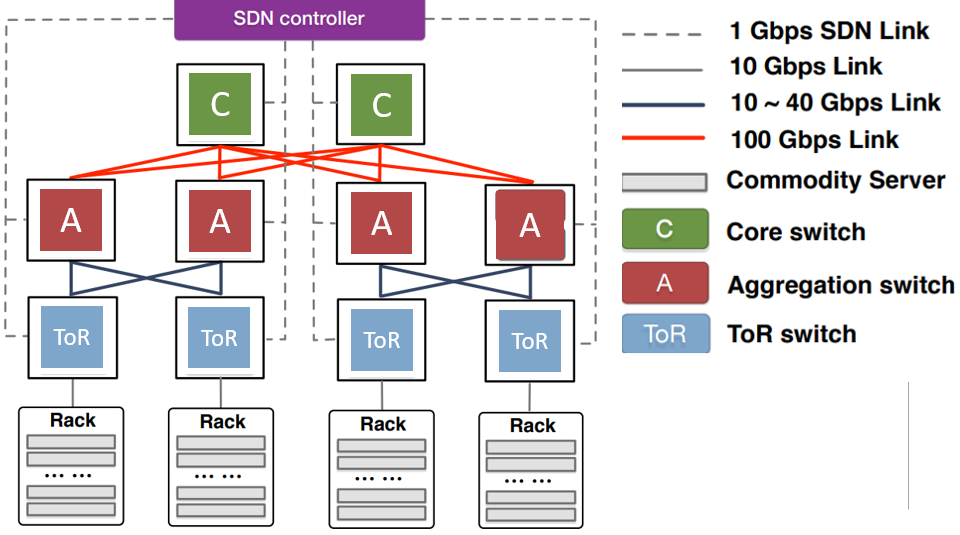
\includegraphics[width=.6\linewidth, trim=2 3 3 3,clip]{Figures/dc.png}
	\caption{Overview of a typical datacenter network topology.}
	\label{fig:dc}
\end{figure}

\subsection{Datacenter Network Toplogy}
\label{sec:datacenternetwork}
A typical datacenter network has a hierarchical, multi-tiered topology~\cite{Mysore2009PortLandAS,VL2,Roy2015InsideTS,incbricks} (Figure~\ref{fig:dc}). Machines are grouped into \textit{racks}, each connecting to a top-of-rack \textit{(ToR)} switch. ToR switches are connected to multiple upper level devices. In this setting, the communication performance of two end-hosts is affected by where they reside: they enjoy full link bisection bandwidth within a rack, because link capacity is not shared at the rack-level, but if they are on different racks, the communication performance depends on link congestion and oversubscription ratio~\cite{Bilal2012ACS}. In this paper, we use \textit{locality} to refer to the cause of variation in communication performance, which includes: (1) physical topology: the location of the nodes and (2) dynamic network load. Efficient communication requires carefully architecting software to tap into both aspects~\cite{eyeQ, 27Octobe15:online}: solutions that ignore physical topology are subject to long-term communication imbalances, and those that ignore dynamic network load suffer from short-term inefficiencies.
\chapter{\pbox: a Balanced Hardware Design for Parameter Servers at Rack-Scale}
\label{sec:phub}
We now describe \pbox, the solution to inefficient distributed training for clusters with a flat network topology (rack-level). \pbox provides a re-design of a PS at the hardware level, and mostly applies to situations where the user assumes full control over the cluster. We start with the current problem with the PS software and hardware that runs it. When deployed, \pbox serves as a centeralized parameter server in the cluster.

\begin{table}
        \centering
        \footnotesize
	\begin{tabular}{|c|c|c|c|c|}
		\hline
		Network   & CC & CS & NCC & NCS\\
		\hline
		ResNet 269    & 122   & 31   & 140    &  17   \\
		\hline
		Inception & 44   &  11  &  50   &  6  \\
		\hline
		GoogleNet & 40   &  10  &  46   &  6  \\
	
		\hline 
		AlexNet   & 1232  &  308  & 1408    &  176  \\
		\hline
	\end{tabular}
	\caption{Estimated bisection bandwidth (Gbps) lower bound on the PS side for hiding communication latency in a small cluster of 8 nodes with GTX 1080 Ti.}
	\label{table:bwReqDC}
\end{table}

\section{Insufficient Bandwidth and Overprovisioned Compute Resources in Rack-Scale Clusters}
Centralized PSs have lower cost than NCS PSs, and half of the bandwidth stress compared to CS PSs on each interface card. Thus it is desirable to have a centralized reduction entity at rack level. However, scaling a centralized PS to rack scale is challenging~\cite{firecaffe}.
%Because they dedicate their full bandwidth to the PS process, centralized PSs are bandwidth efficient without the extra hardware cost for non-colocated sharded PSs. They are also compute efficient when not overwhelmed~\cite{firecaffe}. However, while optimizations in \mysection\ref{sec:commonOptimizations} benefit sharded servers, they have only limited effect on the throughput of a centralized PS. 
%The root cause is hardware imbalance in resource allocation of the host machine.
The root cause is hardware imbalance in the allocation of computation and communication resources in the host: centralized PSs usually run on the same hardware configuration as a worker, which have only one or two network interfaces. This implies incast congestion from their high bandwidth usage when serving multiple workers, starving the compute units. We profiled the training of multiple DNNs of different model sizes and computation-to-communication ratios. Our setup used 8 workers and 8 CS PSs. We observed \textit{it was nearly impossible to eliminate communication latency in cloud-based training due to limited network bandwidth.} We estimated the minimum bandwidth requirement to fully hide communication latency in the network as follows: given a model size of $M$, and $T$ time for each iteration, with $N$ workers participating, the network should at least be able to send and receive model updates within the computation time (assuming infinitely fast PSs and that sending/receiving could fully overlap). Figure \ref{fig:pssetups} gives an analytical lower bound of \textit{per host bandwidth}, and Table \ref{table:bwReqDC} shows the required bandwidth for various DNNs: DNNs demand more bandwidth than mainstream offers (typically 10 Gbps). 

%Hardware imbalances result from vastly different computation and communication resources in a machine, which is in turn related to how centralized PSs are deployed. Centralized PSs usually run on the same hardware as a worker and have only one or two network interfaces. This implies incast congestion from their high bandwidth usage (Table \ref{table:bwReqDC}) when serving multiple workers, starving the compute units. 

%Existing frameworks also cannot efficiently use full hardware, even if multiple interfaces are present (for example, TensorfFlow and \mxnet can only use multiple interfaces by spawning multiple PS processes), let alone understanding the topology of the underlying hardware to balance workload in each interface, processor core and NUMA domain.

One trivial solution would be to simply use interfaces with higher bandwidth. However, even in the best case, a single network interface is not capable of saturating memory or PCIe bandwidth. A single network interface also causes serialization delay and further imbalance across NUMA domains in a typical server. %It is not possible to fully utilize the entire server without balancing these resources.

%The solution may seem trivial: just add more interfaces, or use interfaces with higher capacity. These, however, are not enough. First, most parameter server implementations (TensorFlow, \mxnet and etc) do not allow use of multiple interfaces in a single parameter server process instance. To support that, the software stack must understand the topology of the underlying system and produce a balanced scheme across multiple interfaces with minimum polling overhead; second, existing single interface is unlikely able to match the memory bandwidth nor the PCIe bandwidth, and they can still cause serialization delay, further causing imbalance across NUMA domains on typical server systems.

%Software changes alone is not enough to scale training throughput on a typical centralized parameter server, because the hardware offered is inbalanced itself: the provisioned network bandwidth is vastly smaller than available memory bandwidth.
%Therefore, a hardware design that optimizes balance is needed to fully scale a centralized PS. 

\section{\pbox Architecture}
This section describes \pbox, our \textit{balanced parameter exchange system}. We maintain that a centralized system, when architected properly, can provide high throughput, low latency, sufficient scalability for a rack, and low cost. We focus on the hardware side of \pbox, and in the next section, we detail the software side.

We prototyped \pbox using an off-the-shelf server platform that was configured to our requirements. Our goal was to balance IO and memory bandwidth; our prototype system had memory bandwidth of 120 GB/s and theoretical overall bidirectional IO bandwidth of 140 GB/s. To fully utilize resources, \pbox needed a matching network capability, which we provided by using multiple network interfaces. Figure \ref{fig:phub} shows the resulting \pbox design. The system includes 10 network interfaces, each of 56 Gbps link speed, connected to a switch. This uses all PCIe bandwidth on our dual socket prototype and provides roughly 136 GB/s bandwidth once IB and PCIe framing overheads are taken into account, balancing IO and memory bandwidth.

\begin{figure}[t!]
	\centering
	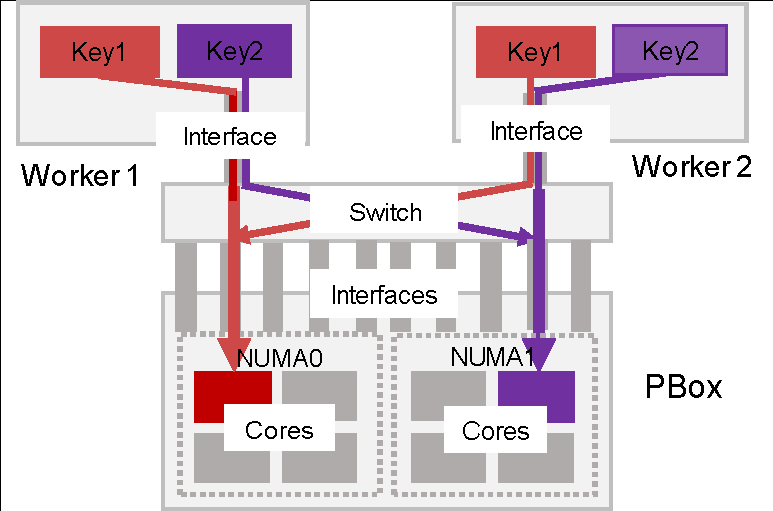
\includegraphics[width=.6\linewidth,trim=2 1 1 1,clip]{Figures/PHubOverview.pdf}
	\caption{The \pbox architecture}
	\label{fig:phub}
\end{figure}



\begin{figure}[t!]
	\centering
	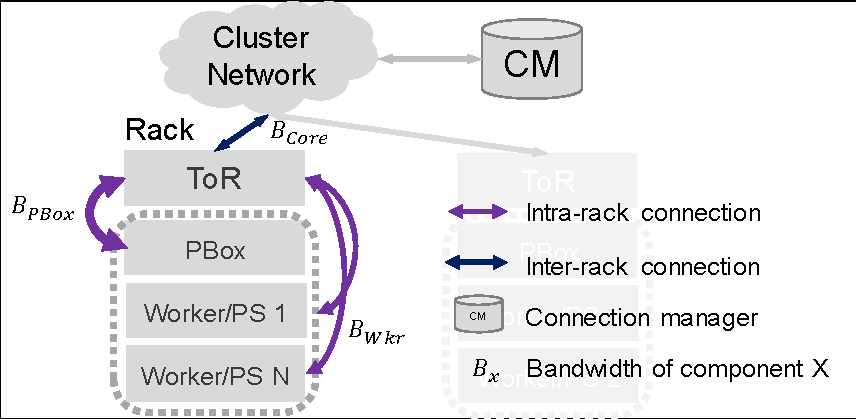
\includegraphics[width=.6\linewidth,trim=3 1 1 2,clip]{Figures/PBoxDeployment.pdf}
	\caption{\pbox deployment scheme}
	\label{fig:pBoxDeployment}
\end{figure}


\section{Multi-Rack Deployment and Topology-Aware Reduction}
\label{sec:hierarchicalReduction}
When needed, \pbox can be used to upscale distributed training to datacenter levels. To extend service coverage of a single \pbox device, we associate a \pbox with a ToR during deployment, for two reasons. First, full bisection bandwidth is achievable for machines in the same rack, making it ideal for a central reduction entity as \pbox, while oversubscription occurs between the ToR and the cluster network. Second, as we show later, a single \pbox has enough scalability for a typical rack of worker machines.

When provisioned in each rack (Figure \ref{fig:pBoxDeployment}), \pbox{}es can form an array of sharded PSs, or run a \textit{hierarchical reduction} algorithm for a training task that spans multiple racks through the coordination of a connection manager. Hierarchical reduction works in three steps: first, each \pbox centrally aggregates gradient updates from workers in the same rack; then, the \pbox{} nodes start cross-rack aggregation and compute globally aggregated gradients; finally, each per-rack \pbox runs an optimizer on this gradient and broadcasts the new weights back to local workers.

Hierarchical reduction trades off more rounds of communication for lower cross-rack traffic ($1/N$ with N-worker racks). We can determine when hierarchical reduction is potentially beneficial with the simple model below:
%\[	max(\frac{N-1}{B_{bn}}, \frac{1}{B_{Wkr}})  > max(\frac{1}{B_{Wkr}}, \frac{N}{B_{PBox}}) + C\]

\begin{align*}
	 \frac{N(R-1)}{RB_{Core}} >  max(\frac{N}{B_{PBox}}, \frac{1}{B_{Wkr}}) + C
\end{align*}
%\[\]

where $B_{PBox}, B_{Core}$ and $B_{Wkr}$ are the bandwidths of a \pbox, the network core, and a worker, and $R$ is the number of racks. When the condition is true, this means the time to perform cross-rack transfer is larger than the added latency of a two-level reduction, which consists of a per-rack local aggregation that happens in parallel and an inter-rack communication (with cost $C$) done with either sharded PSs ($C=\frac{r-1}{rB_{bn}}$, where $B_{bn} = min(B_{PBox}, B_{Core})$) or a collectives operation (e.g., $C\approx\frac{r-1}{rB_{bn}}$ with racks forming a ring). $C$ can be directly measured, and $B_{Core}$ can be effectively probed by using~\cite{hu2002estimating,hu2003evaluation}.

\bibliographystyle{plain}
\bibliography{uwthesis}

\end{document}
